\documentclass[a4paper]{article}
\usepackage[utf8]{inputenc}
\usepackage[polish]{babel}
\usepackage{polski}
%\usepackage{indentfirst}
%\usepackage{default}
%\usepackage{graphicx}
%\usepackage{inconsolata}
\usepackage{geometry}
\usepackage{graphicx}
\usepackage{array}
\usepackage{enumerate}
\usepackage{enumitem}
%\usepackage{parskip}
%\setlength{\parskip}{1ex}
\usepackage[T1]{fontenc}
\usepackage{color}
\definecolor{bluekeywords}{rgb}{0.13,0.13,1}
\definecolor{greencomments}{rgb}{0,0.5,0}
\definecolor{redstrings}{rgb}{0.9,0,0}

\begin{document}

\begin{titlepage}
    \begin{center}
        \bfseries
        \huge Politechnika Wrocławska
        \vskip.2in
        \textsc{\LARGE Wydział Elektroniki}
        \vskip.2in
        \Large Bazy Danych
        \vskip1.5in
        \emph{\huge System szeregowania zadań na linii produkcyjnej }
    \end{center}

    \vskip1.4in

    \begin{minipage}{.50\textwidth}
        \begin{flushleft}
            \bfseries\large Prowadzący:\par \emph{Dr inż. Grzegorz Mzyk}
        \end{flushleft}
    \end{minipage}
    %\hskip.4\textwidth
    \begin{minipage}{.45\textwidth}
        \begin{flushright}
            \bfseries\large Studenci:\par \emph{ Adam Balawender \\ Daniel Duchnicki \\ Adam Prochownik }
        \end{flushright}
    \end{minipage}

    \vskip1.3in

    \centering
    \bfseries
    \Large Semestr letni 2014/2015


\end{titlepage}

\section{Opis metod działających na bazie danych}

\subsection{Baza firm}
\begin{itemize}
    \item Dodaj firmę - dodaje firmę    \\
        param[in] nazwa - nazwa firmy   \\
        param[in] adres  - adres firmy    \\
        param[out] id   - identyfikator \\
    \item Usuń firmę - usuwa firmę i~wszystkie jej zadania \\
        param[in] id  - identyfikator firmy \\
    \item Edytuj firmę - zmienia dane firmy \\
        param[in] id - identyfikator firmy  \\
        param[in] nazwa - nowa nazwa firmy  \\
        param[in] adres - nowy adres firmy
\end{itemize}

\subsection{Zadania}
\begin{itemize}
    \item Dodaj zadanie - dodaje zadanie, uzupełnia datę przyjęcia, uzupełnia operacje przypisane do zadania \\
        param[in] firma - identyfikator firmy                       \\
        param[in] operacje - lista operacji związanych z~zadaniem   \\
        param[out]id - identyfikator utworzonego zadania            \\
    \item Usuń zadanie - usuwa pojedyncze zadanie, razem z wszystkimi przypisanymi do niego operacjami, znalezionymi permutacjami oraz przypisanymi maszynami.             \\
        param[in] id - identyfikator zadania
\end{itemize}

\subsection{Maszyny}
\begin{itemize}
    \item Dodaj maszynę - dodaję nową maszynę do systemu.   \\
        param[in] opis - opis maszyny                       \\
        param[out] id - identyfikator utworzonej maszyny    \\
    \item Usuń maszynę - usuwa maszynę, razem ze wszystkimi procesami i zadaniami, które ją wykorzystują \\
        param[in] id - identyfikator maszyny do usunięcia   \\
    \item Sprawdź\_czy\_używana - sprawdza, czy istnieją zadania przypisane do maszyny \\
        param[in] id - identyfikator maszyny                \\
\end{itemize}

\subsection{Uszeregowanie}
\begin{itemize}
    \item Policz permutację - oblicza permutację i uzupełnia datę obliczenia w tabeli zadania \\
        param[in] id - identyfikator zadania \\
        param[out] kolejność - obliczona permutacja
\end{itemize}

\section{Diagram ERD}
\begin{figure}[h]
    \centering
    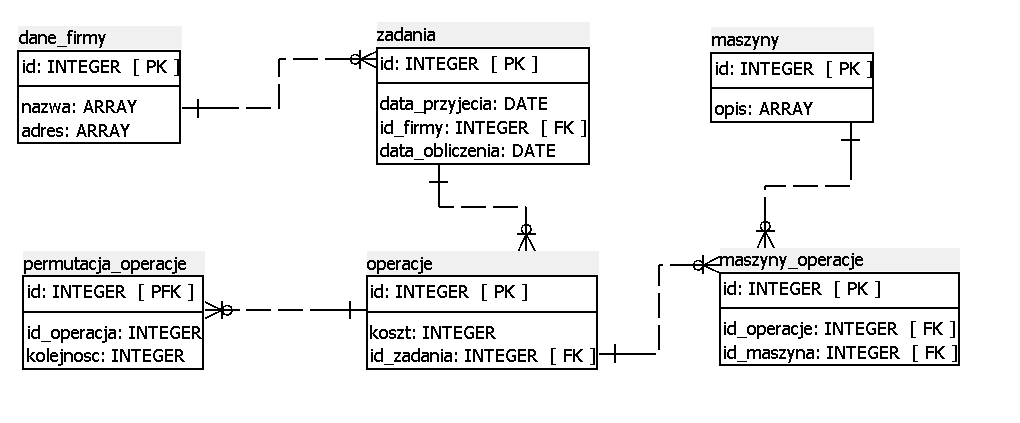
\includegraphics[width=\textwidth]{erd.png}
    \caption{Diagram ERD}
    \label{fig:erd_image}
\end{figure}
\end{document}
